% Created 2018-10-29 ma 10:03
% Intended LaTeX compiler: pdflatex
\documentclass{article}

%%%% settings when exporting code %%%% 

\usepackage{listings}
\lstset{
backgroundcolor=\color{white},
basewidth={0.5em,0.4em},
basicstyle=\ttfamily\small,
breakatwhitespace=false,
breaklines=true,
columns=fullflexible,
commentstyle=\color[rgb]{0.5,0,0.5},
frame=single,
keepspaces=true,
keywordstyle=\color{black},
literate={~}{$\sim$}{1},
numbers=left,
numbersep=10pt,
numberstyle=\ttfamily\tiny\color{gray},
showspaces=false,
showstringspaces=false,
stepnumber=1,
stringstyle=\color[rgb]{0,.5,0},
tabsize=4,
xleftmargin=.23in,
emph={anova,apply,class,coef,colnames,colNames,colSums,dim,dcast,for,ggplot,head,if,ifelse,is.na,lapply,list.files,library,logLik,melt,plot,require,rowSums,sapply,setcolorder,setkey,str,summary,tapply},
emphstyle=\color{blue}
}

%%%% packages %%%%%

\usepackage[utf8]{inputenc}
\usepackage[T1]{fontenc}
\usepackage{lmodern}
\usepackage{textcomp}
\usepackage{color}
\usepackage{enumerate}
\usepackage{graphicx}
\usepackage{grffile}
\usepackage{wrapfig}
\usepackage{rotating}
\usepackage{longtable}
\usepackage{multirow}
\usepackage{multicol}
\usepackage{changes}
\usepackage{pdflscape}
\usepackage{geometry}
\usepackage[normalem]{ulem}
\usepackage{amssymb}
\usepackage{amsmath}
\usepackage{amsfonts}
\usepackage{dsfont}
\usepackage{textcomp}
\usepackage{array}
\usepackage{ifthen}
\usepackage{hyperref}
\usepackage{natbib}
%
%%%% additional packages %%%%
%
\usepackage{authblk}
\RequirePackage{fancyvrb}
\DefineVerbatimEnvironment{verbatim}{Verbatim}{fontsize=\small,formatcom = {\color[rgb]{0.5,0,0}}}
\RequirePackage{epstopdf} % to be able to convert .eps to .pdf image files
%
%%%% additional latex commands %%%%
%
\date{}
\title{Univariate test vs multivariate test}
\hypersetup{
 colorlinks=true,
 citecolor=[rgb]{0,0.5,0},
 urlcolor=[rgb]{0,0,0.5},
 linkcolor=[rgb]{0,0,0.5},
 pdfauthor={},
 pdftitle={Univariate test vs multivariate test},
 pdfkeywords={},
 pdfsubject={},
 pdfcreator={Emacs 25.2.1 (Org mode 9.0.4)},
 pdflang={English}
 }
\begin{document}

\maketitle
\lstset{language=r,label= ,caption= ,captionpos=b,numbers=none}
\begin{lstlisting}
library(mvtnorm)
library(data.table)
library(ggplot2)
library(ggforce) # install.packages("ggforce")
\end{lstlisting}

\section{One-dimensional test}
\label{sec:orgab822a9}

Create a 1D-grid of values corresponding to the possible values of the 1D statistic test:
\lstset{language=r,label= ,caption= ,captionpos=b,numbers=none}
\begin{lstlisting}
grid1D <- seq(-3,3,0.025)
\end{lstlisting}

The rejection region at 5\% is defined by the 0.025 and 0.975 quantiles of the normal distribution:
\lstset{language=r,label= ,caption= ,captionpos=b,numbers=none}
\begin{lstlisting}
rejection1D <- c(qnorm(0.025), qnorm(0.975))
rejection1D
\end{lstlisting}

\begin{verbatim}
[1] -1.959964  1.959964
\end{verbatim}

\lstset{language=r,label= ,caption= ,captionpos=b,numbers=none}
\begin{lstlisting}
plot(grid1D, dnorm(grid1D), type = "o", xlab = "value of the statistic test", 
	 ylab = "density")
abline(v = rejection1D, col = "red")
legend("topright", col = "red", lty = 1, legend = "rejection zone", bty = "n")
\end{lstlisting}

We can then plot the values of the statistic tests and the rejection region:
\begin{center}
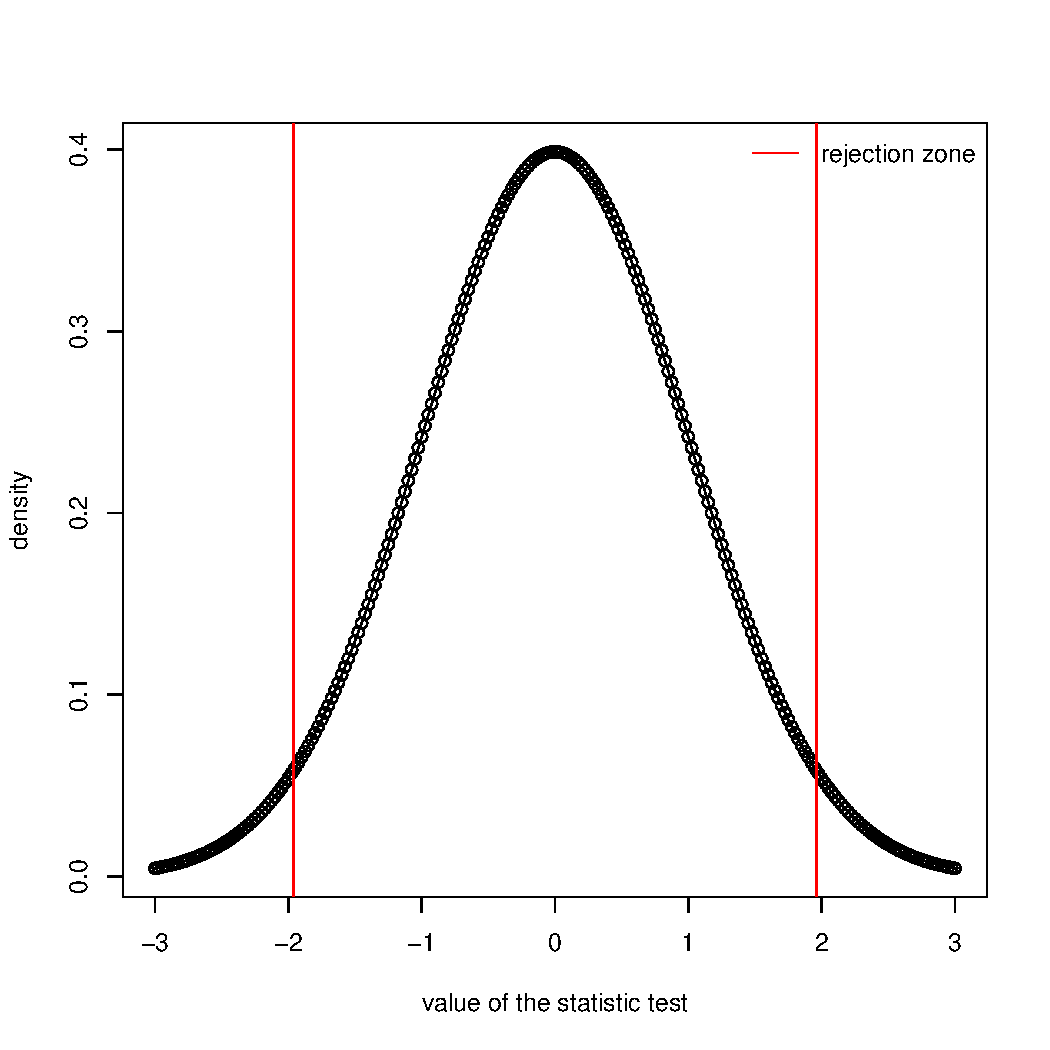
\includegraphics[width=0.7\textwidth]{figures/1D-test.pdf}
\end{center}




\section{2 dimensional test}
\label{sec:org4988089}

Create a 2D-grid of values corresponding to the possible values of the 2D statistic test:
\lstset{language=r,label= ,caption= ,captionpos=b,numbers=none}
\begin{lstlisting}
grid2D <- as.data.table(expand.grid(beta1 = grid1D, beta2 = grid1D))
grid2D[, density := dmvnorm(cbind(beta1, beta2))]
range(grid2D$density)
\end{lstlisting}

\begin{verbatim}
[1] 1.964128e-05 1.591549e-01
\end{verbatim}

If we would do two univariate tests (not accounting for multiple
testing), the rejection region at 5\% would be a square whose size is
defined the 0.025 and 0.975 quantiles of the normal distribution:
\lstset{language=r,label= ,caption= ,captionpos=b,numbers=none}
\begin{lstlisting}
rejection2D.2uni <- data.table(xmax = qnorm(0.975, mean = 0, sd = 1),
							   ymax = qnorm(0.975, mean = 0, sd = 1),
							   xmin = qnorm(0.025, mean = 0, sd = 1),
							   ymin = qnorm(0.025, mean = 0, sd = 1))
rejection2D.2uni
\end{lstlisting}

\begin{verbatim}
       xmax     ymax      xmin      ymin
1: 1.959964 1.959964 -1.959964 -1.959964
\end{verbatim}

When we account for multiple comparison we get:
\lstset{language=r,label= ,caption= ,captionpos=b,numbers=none}
\begin{lstlisting}
rejection2D.2uniadj <- data.table(xmax = qmvnorm(0.95, mean = c(0,0), sigma = diag(1,2), tail = "both")$quantile,
								  ymax = qmvnorm(0.95, mean = c(0,0), sigma = diag(1,2), tail = "both")$quantile,
								  xmin = -qmvnorm(0.95, mean = c(0,0), sigma = diag(1,2), tail = "both")$quantile, 
								  ymin = -qmvnorm(0.95, mean = c(0,0), sigma = diag(1,2), tail = "both")$quantile)
rejection2D.2uniadj
\end{lstlisting}

\begin{verbatim}
       xmax     ymax      xmin      ymin
1: 2.236422 2.236422 -2.236422 -2.236422
\end{verbatim}

If we do a bivariate test, the rejection region at 5\% would be a
circle whose radius is the 0.95 quantile of a chi-squared distribution
with 2 degrees of freedom:
\lstset{language=r,label= ,caption= ,captionpos=b,numbers=none}
\begin{lstlisting}
rejection2D.chisq <- sqrt(qchisq(0.95, df = 2))
rejection2D.chisq
\end{lstlisting}

\begin{verbatim}
[1] 2.447747
\end{verbatim}

\lstset{language=r,label= ,caption= ,captionpos=b,numbers=none}
\begin{lstlisting}
gg2D <- ggplot() + labs(x=expression(beta[1]), y=expression(beta[2]))
gg2D <- gg2D + geom_raster(data = grid2D,aes(x=beta1, y=beta2, fill = density))
gg2D <- gg2D + scale_fill_gradient(low="white", high="blue")

## gg2D <- gg2D + geom_rect(data = rejection2D.2adj, 
##                          aes(xmin = xmin, xmax = xmax, ymin = ymin, ymax = ymax, 
##                              colour = "2 univariate Wald tests (non-adjusted)"), 
##                          size = 2,
##                          fill  = NA) 
gg2D <- gg2D + geom_rect(data = rejection2D.2uniadj, 
						 aes(xmin = xmin, xmax = xmax, ymin = ymin, ymax = ymax, 
							 colour = "2 univariate Wald tests (adjusted)"), 
						 size = 2,
						 fill  = NA) 
gg2D <- gg2D + geom_circle(aes(x0=0, y0=0, r = rejection2D.chisq, 
							   color = "1 Chi-2 test"),
						   size = 2)
gg2D <- gg2D + labs(color = "critical quantile")
gg2D
\end{lstlisting}

\begin{center}
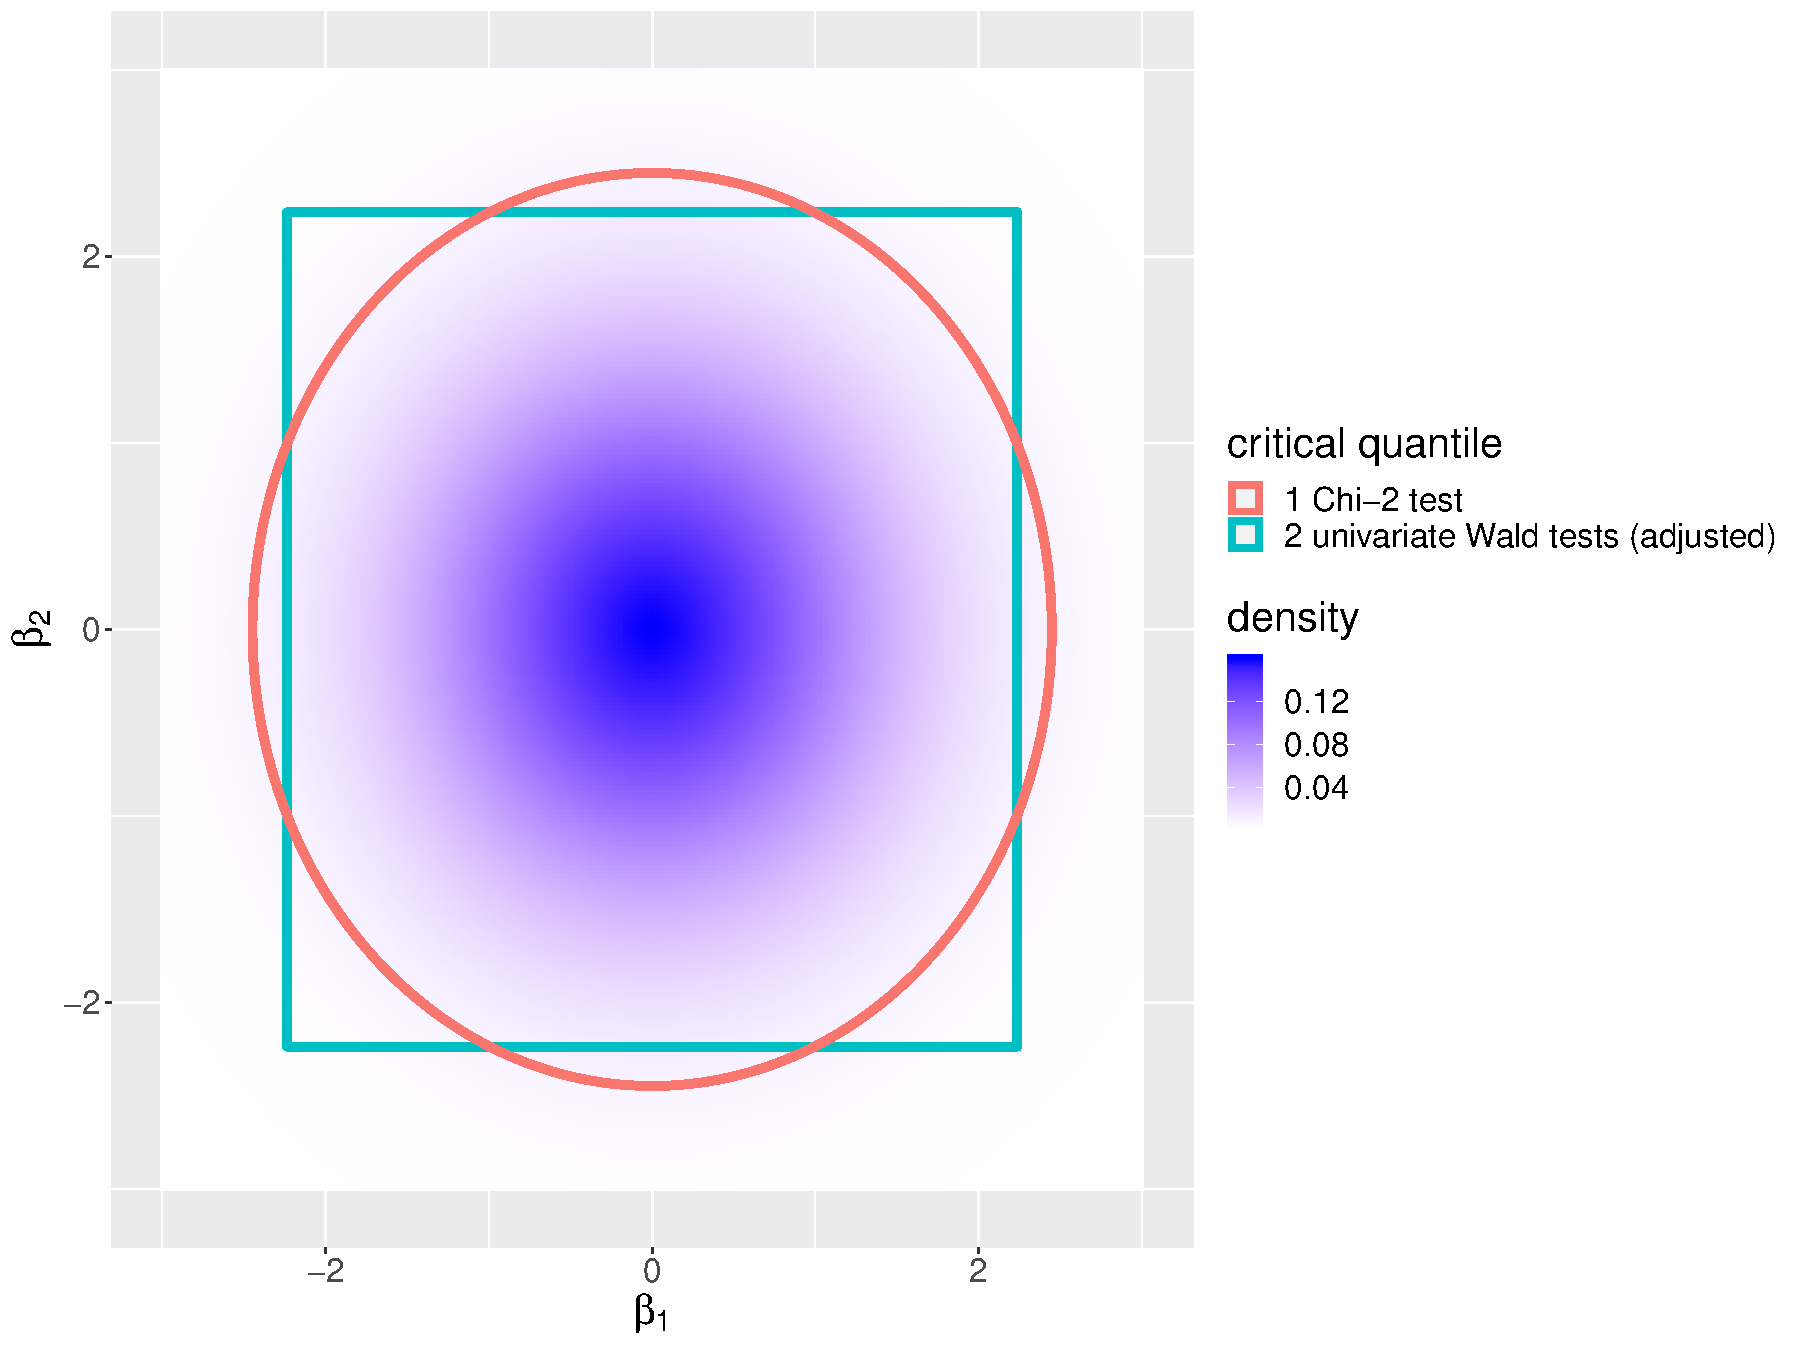
\includegraphics[width=.9\linewidth]{./figures/2D-test.pdf}
\end{center}
\end{document}